% \documentclass{beamer}
\documentclass[xcolor=dvipsnames]{beamer}
%% \usecolortheme[named=Blue]{structure}
\setbeamersize{text margin left=30mm, text margin right=30mm}
\useoutertheme{infolines}
%% \usetheme[height=7mm]{Rochester}
\usetheme{Pittsburgh}
\setbeamertemplate{items}[ball]
\setbeamertemplate{blocks}[rounded][shadow=true]
\setbeamertemplate{navigation symbols}{}

\usepackage[utf8x]{inputenc}
\usepackage{default}
\usepackage[english]{babel}
\usepackage{geometry}
%% \usepackage{fullpage}
\usepackage{amsmath, amsthm, amssymb}
\usepackage{listings}
\usepackage{pxfonts}
%% \usepackage{color}
%% \usepackage{graphicx}
%% \usepackage{natbib}
%% \usepackage{array}
%% \usepackage{booktabs}
%% \usepackage{tabu}
%% \usepackage[utf8]{inputenc}
%% \usepackage{fancyhdr}
%% \usepackage{float}
%% \usepackage{subfigure}
%% \usepackage{titlesec}

\renewcommand{\chaptername}{}
\renewcommand{\bibname}{References}
\newcommand{\pluseq}{\:+\!\!=}
\newcommand{\minuseq}{\:-\!\!=}
\newcommand{\mrm}[1]{\mathrm{#1}}
\newcommand{\bsym}[1]{\boldsymbol{#1}}
\newcommand{\abs}[1]{\lvert#1\rvert}
\newcommand{\norm}[1]{\lVert#1\rVert}

\setcounter{MaxMatrixCols}{20}

\def\CCT{{C\nolinebreak[4]\hspace{-.05em}\raisebox{.4ex}{\tiny\bf ++}}}
\def\CC{{C\nolinebreak[4]\hspace{-.05em}\raisebox{.4ex}{\small\bf ++}}}


\definecolor{lstgray}{gray}{0.93}
\lstset{ %
  escapechar=@,
  language=C++,
  basicstyle=\footnotesize\ttfamily,
  %% basicstyle=\ttfamily,
  %% keywordstyle=\color{blue}\ttfamily,
  keywordstyle=\bfseries,
  stringstyle=\color{red}\ttfamily,
  commentstyle=\color{OliveGreen}\ttfamily,
  morecomment=[l][\color{red}]{\#},
  backgroundcolor=\color{lstgray},
  %% keywordstyle=\color{red},
  frame=f,
  frameround=ffff,
  tabsize=2,
  breaklines=true,
  breakatwhitespace=false,
  showspaces=false,
  showstringspaces=false,
  xleftmargin=5pt,
  xrightmargin=5pt,
  morekeywords={in,out,ref,auto,inout,import,ushort,scope,exit,mixin,decltype,varid,sizeof}
}

\def\redcolor{\color{red}}
\def\bluecolor{\color{blue}}
\def\blackcolor{\color{black}}
\def\graycolor{\color{gray}}
\def\greencolor{\color{OliveGreen}}


\def\sectionname{\translate{Section}}
\def\insertsectionnumber{\arabic{section}}
\setbeamertemplate{section page}
{
  \begin{centering}
    \begin{beamercolorbox}[sep=4pt,center]{part title}
      \usebeamerfont{section title}\insertsection\par
    \end{beamercolorbox}
  \end{centering}
}
\def\sectionpage{\usebeamertemplate*{section page}}


\AtBeginSection{\frame{\sectionpage}}

\usepackage{caption}
\captionsetup[figure]{labelformat=empty}


\title{Computation}
\subtitle{Abstraction and Implementation}
\author{Dominic Jones}
%% \institute{Netherhall House, London}
%% \date{November 2017}
\date{}


\begin{document}
\begin{frame}[plain]
  \titlepage
\end{frame}


\section{CPU - Logic - Transistor}


\begin{frame}{Intel 4004}
\begin{figure}
  \centering
  \begin{columns}
    \column{0.5\textwidth}
    \centering
    \caption {4-bit data, 2,300 transistors}
    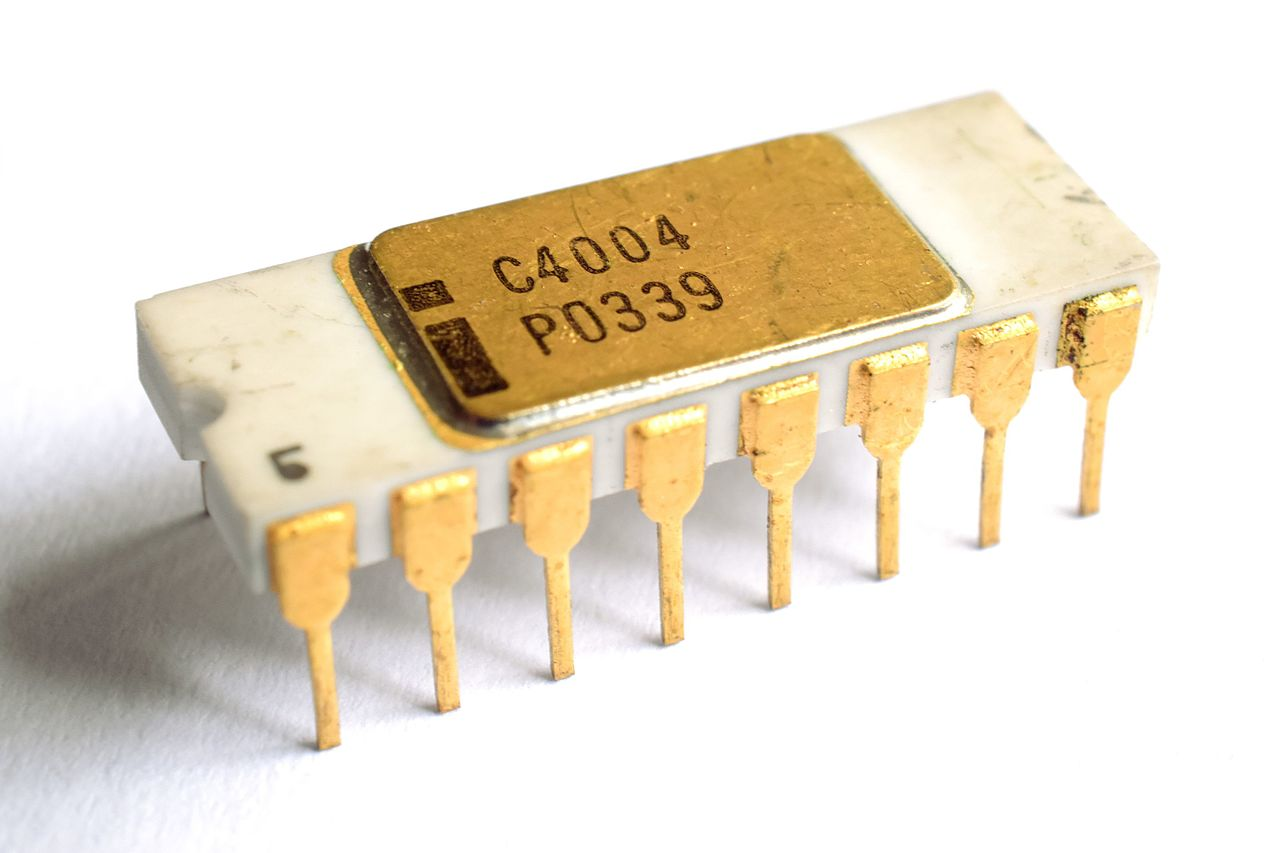
\includegraphics[width=0.99\textwidth]{intel_4004_chip}
    \column{0.5\textwidth}
    \centering
    \caption {16 general registers}
    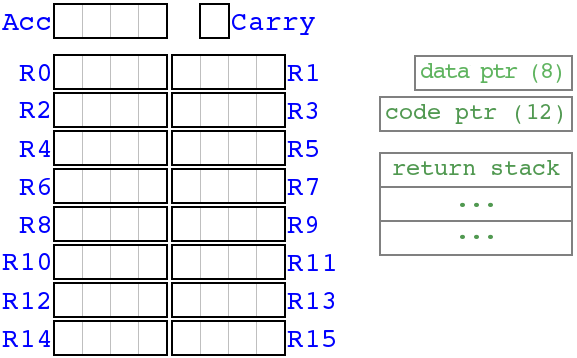
\includegraphics[width=0.99\textwidth]{intel_4004_registers}
  \end{columns}
\end{figure}
Instruction set contains 46 instructions (3,683 in x86-64)
\end{frame}


\begin{frame}{Intel 4004}
\begin{figure}
  \centering
  \caption {Single cycle data path architecture}
  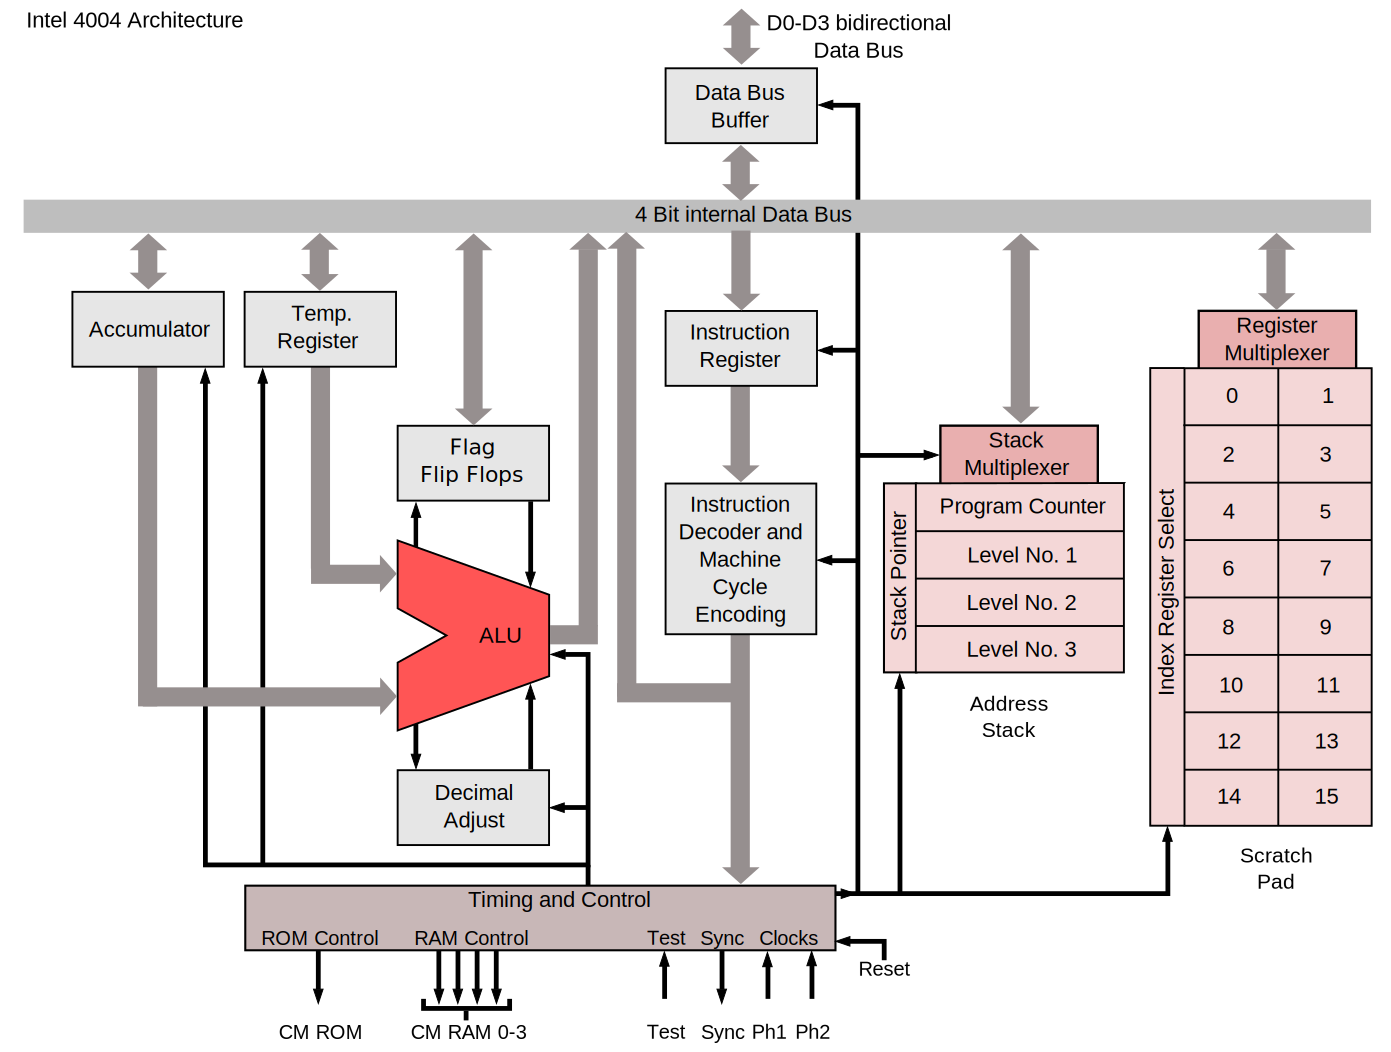
\includegraphics[width=0.7\textwidth]{intel_4004_architecture}
\end{figure}
\end{frame}


\begin{frame}[fragile]
  \frametitle{Intel 4004 Emulator}
  \centering
  {\color{red}59} + {\color{blue}38} = {\color{OliveGreen}91}
\begin{columns}
\column{0.5\textwidth}
\centering
\begin{lstlisting}


@\aftergroup\graycolor@; sum lower digits (9,8)@\aftergroup\blackcolor@
clc    @\aftergroup\graycolor@; car = 0@\aftergroup\blackcolor@
ld  r1 @\aftergroup\graycolor@; acc = r1@\aftergroup\blackcolor@
add r3 @\aftergroup\graycolor@; acc = acc + car + r3@\aftergroup\blackcolor@
xch r1 @\aftergroup\graycolor@; r1  = acc@\aftergroup\blackcolor@

@\aftergroup\graycolor@; sum higher digits (5,3)@\aftergroup\blackcolor@
ld  r0 @\aftergroup\graycolor@; acc = r0@\aftergroup\blackcolor@
add r2 @\aftergroup\graycolor@; acc = acc + car + r2@\aftergroup\blackcolor@
xch r0 @\aftergroup\graycolor@; r0  = acc@\aftergroup\blackcolor@
\end{lstlisting}
\column{0.5\textwidth}
\centering
\begin{lstlisting}
@\aftergroup\graycolor@acc car  r0 r1 r2 r3@\aftergroup\blackcolor@
  x   x   @\aftergroup\redcolor@5  9@\aftergroup\blackcolor@  @\aftergroup\bluecolor@3  8@\aftergroup\blackcolor@

  x   0   5  9  3  8
  9   0   5  9  3  8
  1   1   5  9  3  8
  1   1   5  1  3  8


  5   1   5  9  3  8
  9   0   5  9  3  8
  9   0   @\aftergroup\greencolor@9  1@\aftergroup\blackcolor@  3  8
\end{lstlisting}
\end{columns}
\end{frame}


\begin{frame}{Instructions}
  \begin{figure}
    \centering
    \caption {4-bit ripple carry adder}
    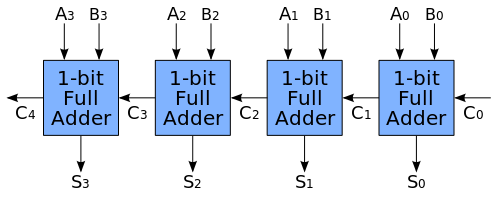
\includegraphics[width=0.6\textwidth]{four_bit_adder}
    \vspace{5mm}
    \caption {1-bit full adder}
    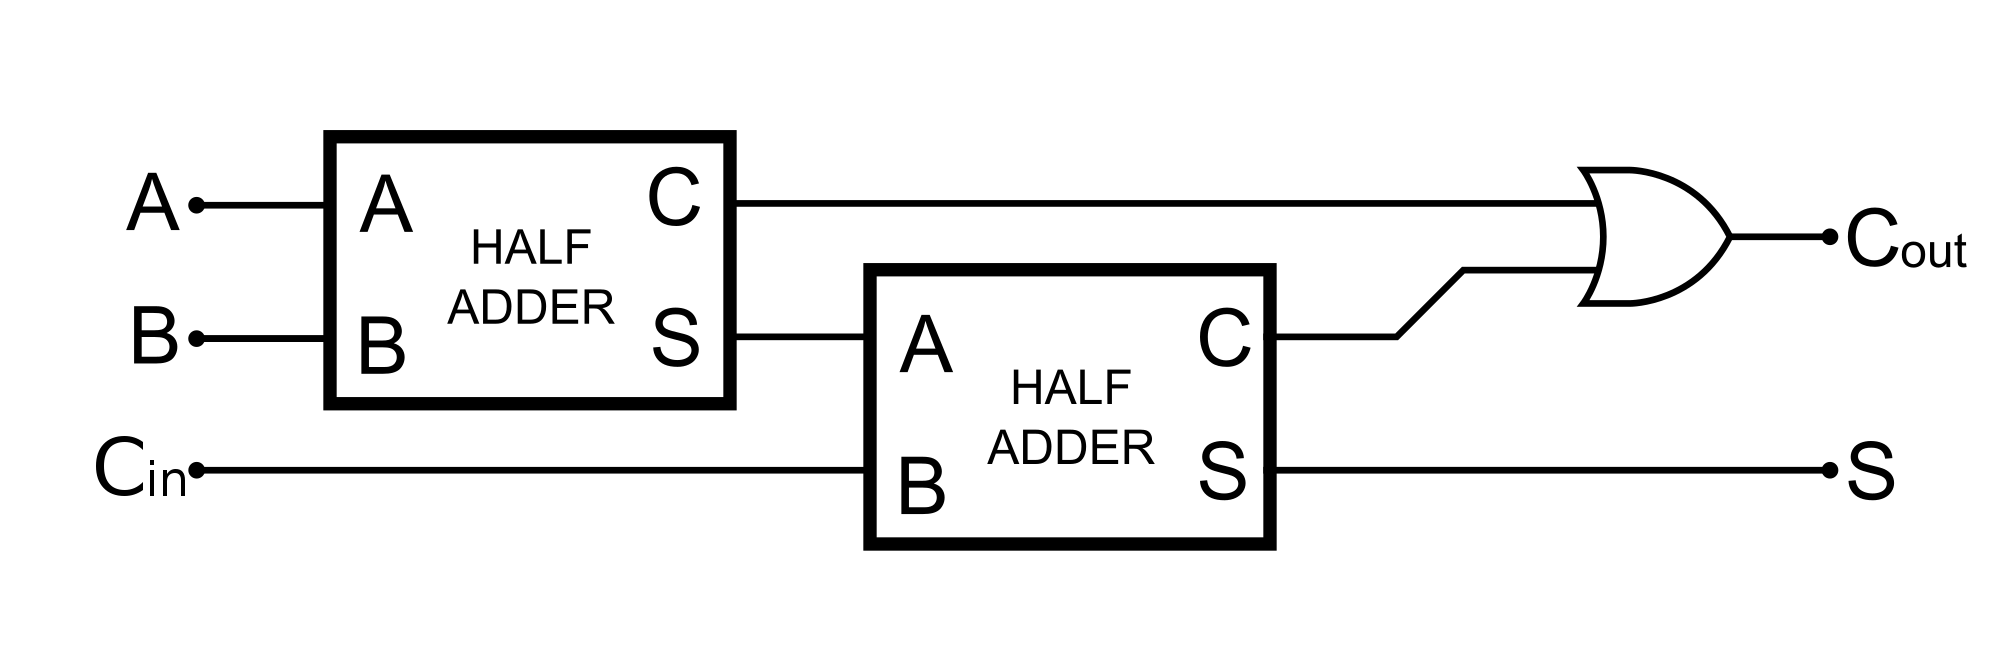
\includegraphics[width=0.6\textwidth]{full_adder}
  \end{figure}
\end{frame}


\begin{frame}{Transistors}
\begin{figure}
  \centering
  \begin{columns}
    \column{0.5\textwidth}
    \centering
    \caption {Half adder}
    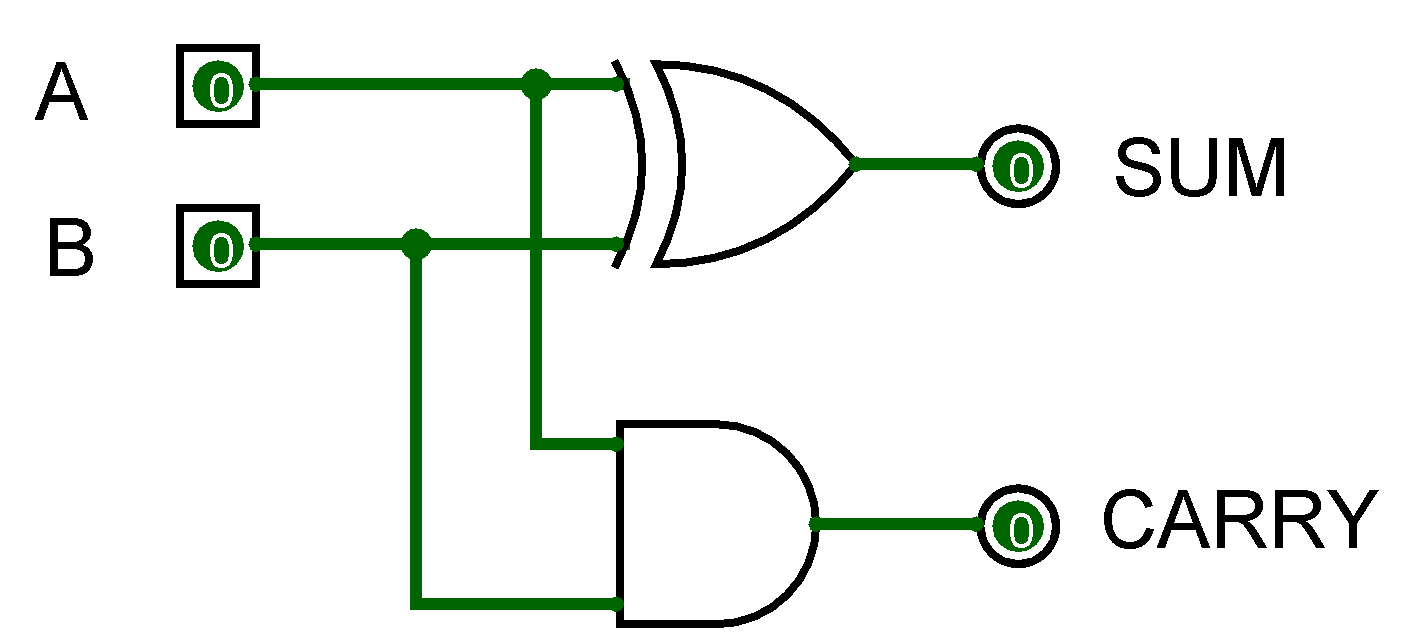
\includegraphics[width=0.9\textwidth]{half_adder}
    \column{0.5\textwidth}
    \centering
    \caption {AND gate circuit}
    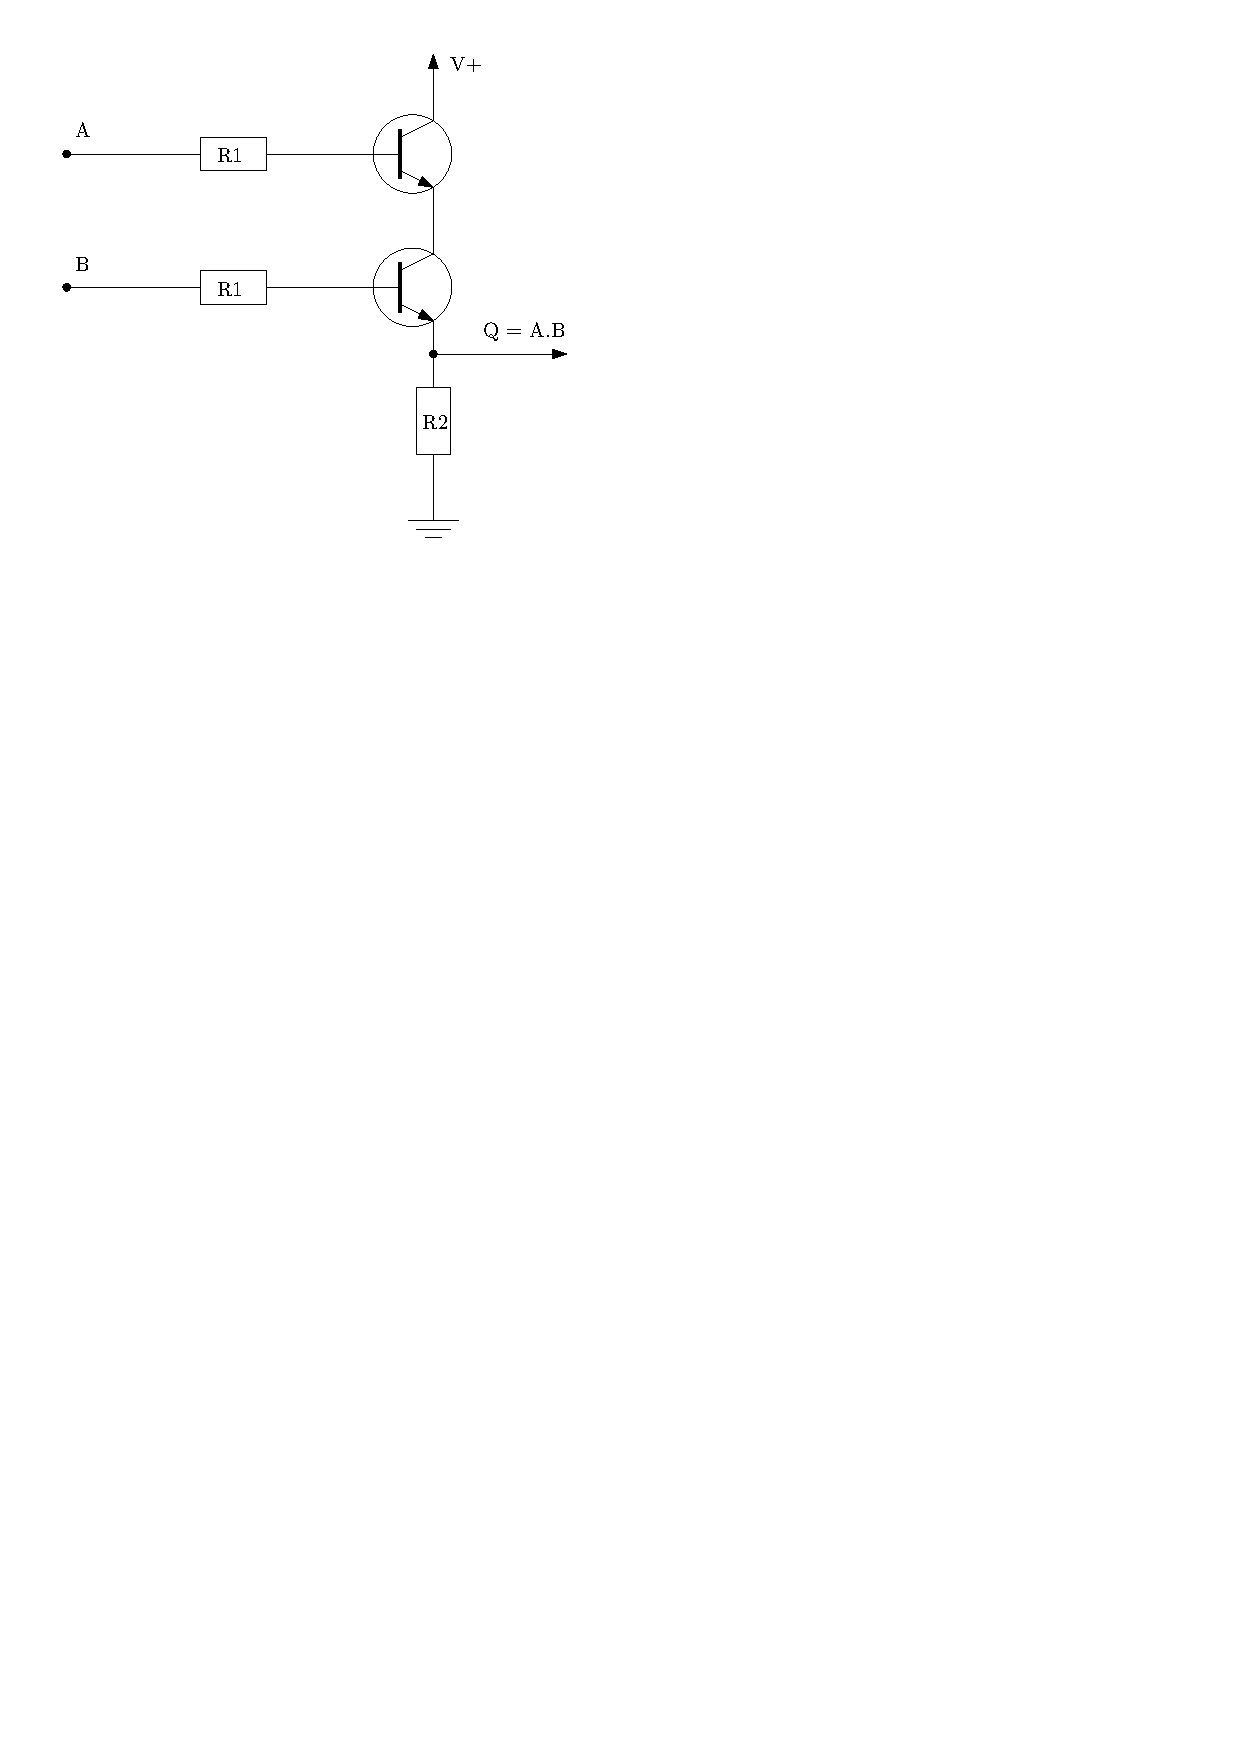
\includegraphics[width=0.9\textwidth]{and_gate_circuit}
  \end{columns}
\end{figure}
\end{frame}


\section{Mathematics - Computation}


\begin{frame}[fragile]
  \frametitle{Intersection of two lines}
\begin{figure}
  \centering
  \begin{columns}
    \column{0.5\textwidth}
    \centering
  \begin{eqnarray*}
    -0.35x + y &=& 2\\
    2.5x - 2y &=& 4
  \end{eqnarray*}
  \begin{eqnarray*}
    \begin{bmatrix}
      -0.35 & 1 \\
      2.5 & -2
    \end{bmatrix}
    \begin{bmatrix}
      x \\
      y
    \end{bmatrix}
    &=&
    \begin{bmatrix}
      2 \\
      4
    \end{bmatrix}
  \end{eqnarray*}
  %% \begin{eqnarray*}
  %%   A x = b
  %% \end{eqnarray*}
  \begin{eqnarray*}
    \begin{bmatrix}
      x \\
      y
    \end{bmatrix}
    &=&
    \begin{bmatrix}
      -0.35 & 1 \\
      2.5 & -2
    \end{bmatrix}^{-1}
    \begin{bmatrix}
      2 \\
      4
    \end{bmatrix}
  \end{eqnarray*}
  %% \begin{eqnarray*}
  %%   x = A^{-1} b
  %% \end{eqnarray*}
  Matrix inverse?
  \column{0.5\textwidth}
    \centering
    %% \caption {Plot of intersecting lines}
    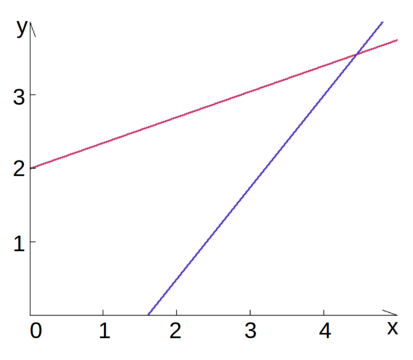
\includegraphics[width=0.9\textwidth]{intersecting_lines}
  \end{columns}
\end{figure}
\end{frame}


\begin{frame}[fragile]
  \frametitle{Division (scalar inverse)}
  \begin{lstlisting}[basicstyle=\tiny\ttfamily]
unsigned divide(unsigned a, unsigned b)
{
  unsigned denom = b, current = 1, result = 0;

  if (denom > a) return 0;
  if (denom == a) return 1;

  while (denom <= a) {
    denom <<= 1;
    current <<= 1;
  }

  denom >>= 1;
  current >>= 1;

  @\aftergroup\redcolor@while@\aftergroup\blackcolor@ (current != 0) {  // n^1
    if (a >= denom) {
      a -= denom;
      result |= current;
    }

    current >>= 1;
    denom >>= 1;
  }

  return result;
}
\end{lstlisting}
\end{frame}


\begin{frame}[fragile]
  \frametitle{Matrix inverse}
\begin{lstlisting}[basicstyle=\tiny\ttfamily]
void inverse(int n, float a[][2*n_max])
{
  for (int i = 0; i < n; i++)
    for (int j = n; j < 2*n; j++)
      a[i][j] = (i == j-n? 1: 0);

  @\aftergroup\redcolor@for@\aftergroup\blackcolor@ (int @\aftergroup\bluecolor@i@\aftergroup\blackcolor@ = 0; i < n; i++) {         // n^1
    float aii = a[i][i];
    for (int j = i; j < 2*n; j++)
      a[i][j] = a[i][j] / aii;

    @\aftergroup\redcolor@for@\aftergroup\blackcolor@ (int @\aftergroup\bluecolor@j@\aftergroup\blackcolor@ = 0; j < n; j++) {       // n^2
      if (i != j) {
        float aji = a[j][i];
        @\aftergroup\redcolor@for@\aftergroup\blackcolor@ (int @\aftergroup\bluecolor@k@\aftergroup\blackcolor@ = 0; k < 2*n; k++)   // n^3
          a[j][k] = a[j][k] - aji * a[i][k];
      }
    }
  }
}
\end{lstlisting}
\end{frame}


\begin{frame}{Simulation: cavity flow}
\begin{figure}
  \centering
  \begin{columns}
    \column{0.5\textwidth}
    \centering
    \caption {Geometry and mesh}
    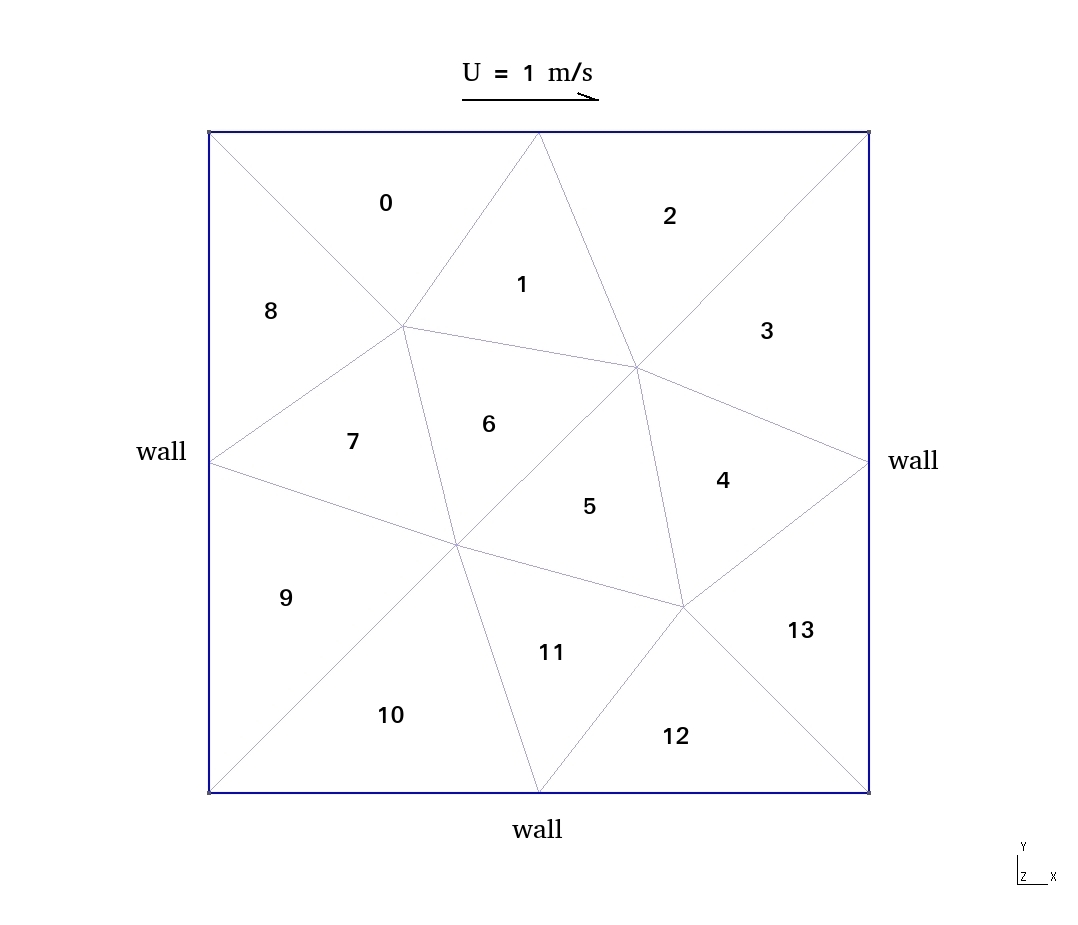
\includegraphics[width=0.99\textwidth]{cavity_2d_tet_i}
    \column{0.5\textwidth}
    \centering
    \caption {Connectivity graph}
    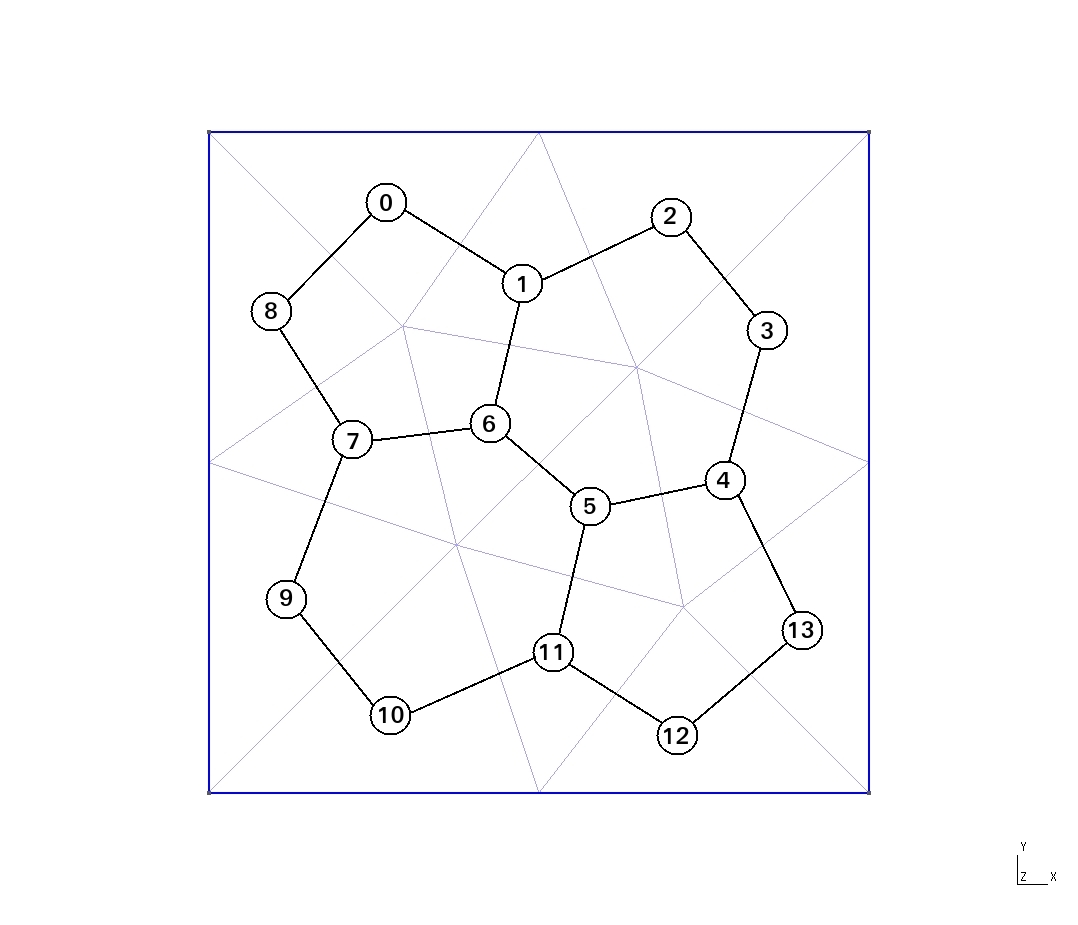
\includegraphics[width=0.99\textwidth]{cavity_2d_tet_d}
  \end{columns}
\end{figure}
\end{frame}


\begin{frame}{Topology Representation}
Symmetric, sparse (48 non-zeros), irregular
  \begingroup
  %% \small
  \tiny
  \centering
\begin{equation*}
\begin{bmatrix}
a_{0,0} & a_{0,1} &  &  &  &  &  &  & a_{0,8} &  &  &  &  & \\
a_{1,0} & a_{1,1} & a_{1,2} &  &  &  & a_{1,6} &  &  &  &  &  &  & \\
& a_{2,1} & a_{2,2} & a_{2,3} &  &  &  &  &  &  &  &  &  & \\
&  & a_{3,2} & a_{3,3} & a_{3,4} &  &  &  &  &  &  &  &  & \\
&  &  & a_{4,3} & a_{4,4} & a_{4,5} &  &  &  &  &  &  &  & a_{4,13} \\
&  &  &  & a_{5,4} & a_{5,5} & a_{5,6} &  &  &  &  & a_{5,11} &  & \\
& a_{6,1} &  &  &  & a_{6,5} & a_{6,6} & a_{6,7} &  &  &  &  &  & \\
&  &  &  &  &  & a_{7,6} & a_{7,7} & a_{7,8} & a_{7,9} &  &  &  & \\
a_{8,0} &  &  &  &  &  &  & a_{8,7} & a_{8,8} &  &  &  &  & \\
&  &  &  &  &  &  & a_{9,7} &  & a_{9,9} & a_{9,10} &  &  & \\
&  &  &  &  &  &  &  &  & a_{10,9} & a_{10,10} & a_{10,11} &  & \\
&  &  &  &  & a_{11,5} &  &  &  &  & a_{11,10} & a_{11,11} & a_{11,12} & \\
&  &  &  &  &  &  &  &  &  &  & a_{12,11} & a_{12,12}  & a_{12,13}\\
&  &  &  & a_{13,4} &  &  &  &  &  &  &  & a_{13,12} &  a_{13,13}
\end{bmatrix}
\end{equation*}
\endgroup
\end{frame}


\begin{frame}[fragile]
  \frametitle{Sparsity and Indirection}
  \begin{itemize}
  \item Dense storage: 196 values, 24\% efficient
  \item Direct access to values
  \end{itemize}
\begin{lstlisting}
  float[13][13] A;
  A[@\aftergroup\redcolor@2@\aftergroup\blackcolor@][@\aftergroup\bluecolor@3@\aftergroup\blackcolor@] = 3.142;
\end{lstlisting}
\vspace{5mm}
  \begin{itemize}
  \item Compressed row storage: 111 values, 56\% efficient
  \item Requires indirection to access values (10x slower)
  \end{itemize}
\begin{lstlisting}
int[15] IA = [0, 3, 7, 10, ...];
int[48] JA = [0, 1, 8,  0, 1, 2, 6,  1, 2, 3,  ...];
float[48] A;

assert(JA[IA[@\aftergroup\redcolor@2@\aftergroup\blackcolor@]+2] == @\aftergroup\bluecolor@3@\aftergroup\blackcolor@);

A[JA[IA[@\aftergroup\redcolor@2@\aftergroup\blackcolor@]+2] = 3.142; // i.e. A[2][3] = 3.142;
\end{lstlisting}
\end{frame}


\begin{frame}{Accuracy}
\begin{figure}
  \centering
  \begin{columns}
    \column{0.5\textwidth}
    \centering
    \caption {Coarse mesh (48 elements)}
    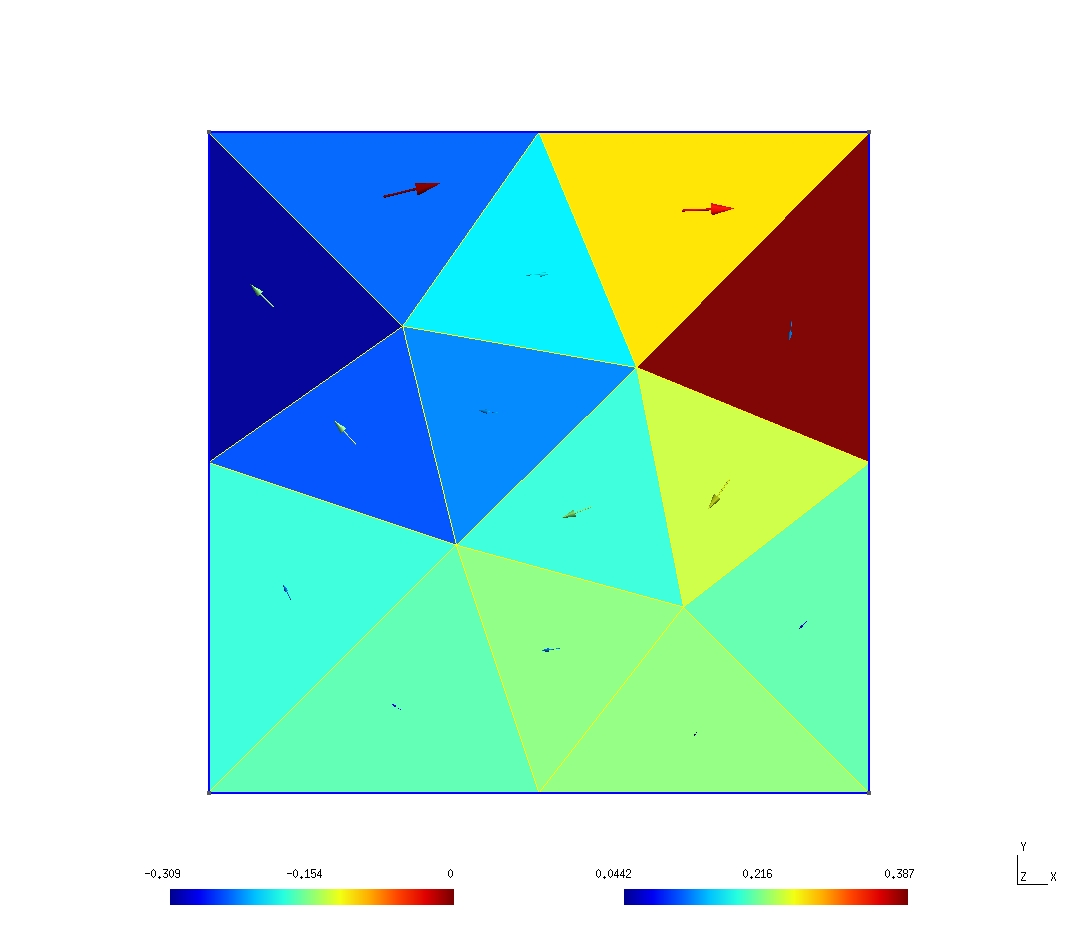
\includegraphics[width=0.99\textwidth]{cavity_2d_tet_coarse}
    \column{0.5\textwidth}
    \centering
    \caption {Fine mesh (132,607 elements)}
    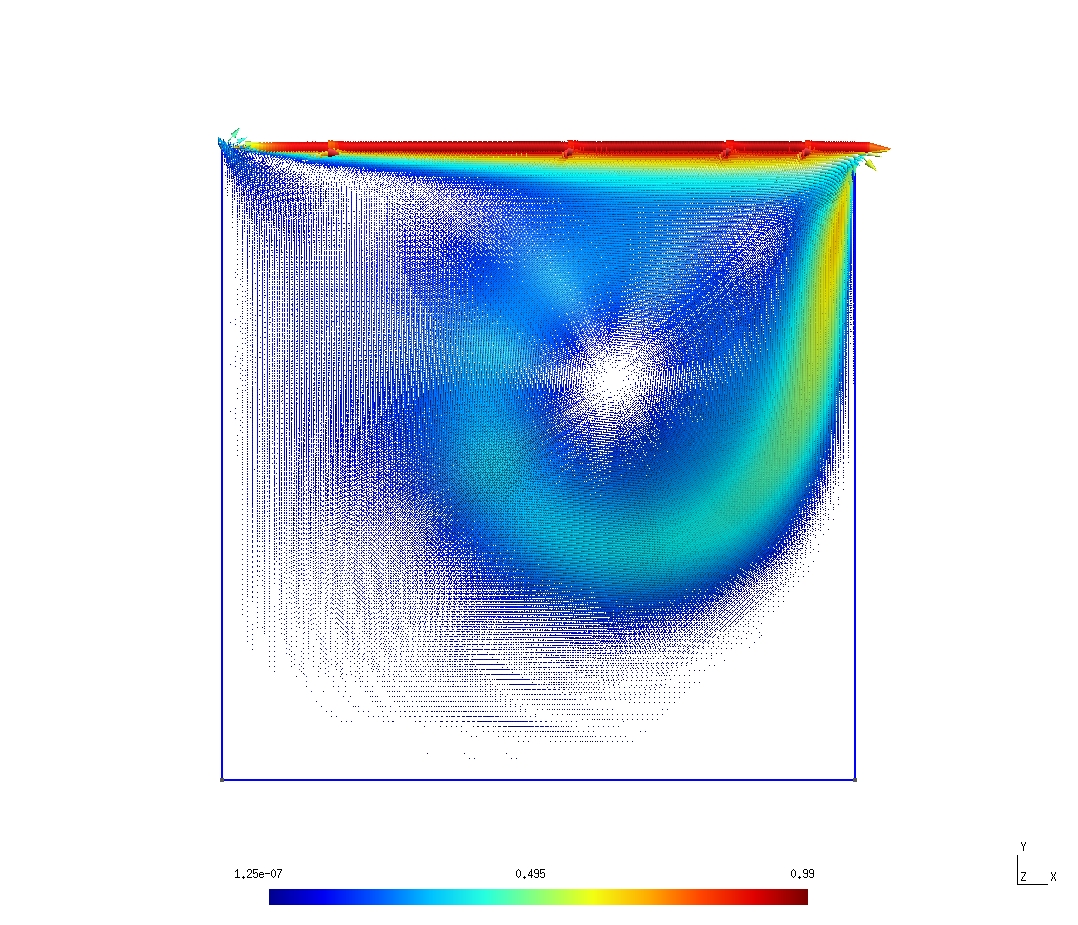
\includegraphics[width=0.99\textwidth]{cavity_2d_tet_fine}
  \end{columns}
\end{figure}
\end{frame}


\begin{frame}{Speed}
  \begin{enumerate}
  \item Partition the mesh into four chunks
  \item Each CPU core computes one chunk
  \item Communication eventually swamps computation
  \end{enumerate}
\begin{figure}
  \centering
  \begin{columns}
    \column{0.5\textwidth}
    \centering
    %% \caption {Cavity flow}
    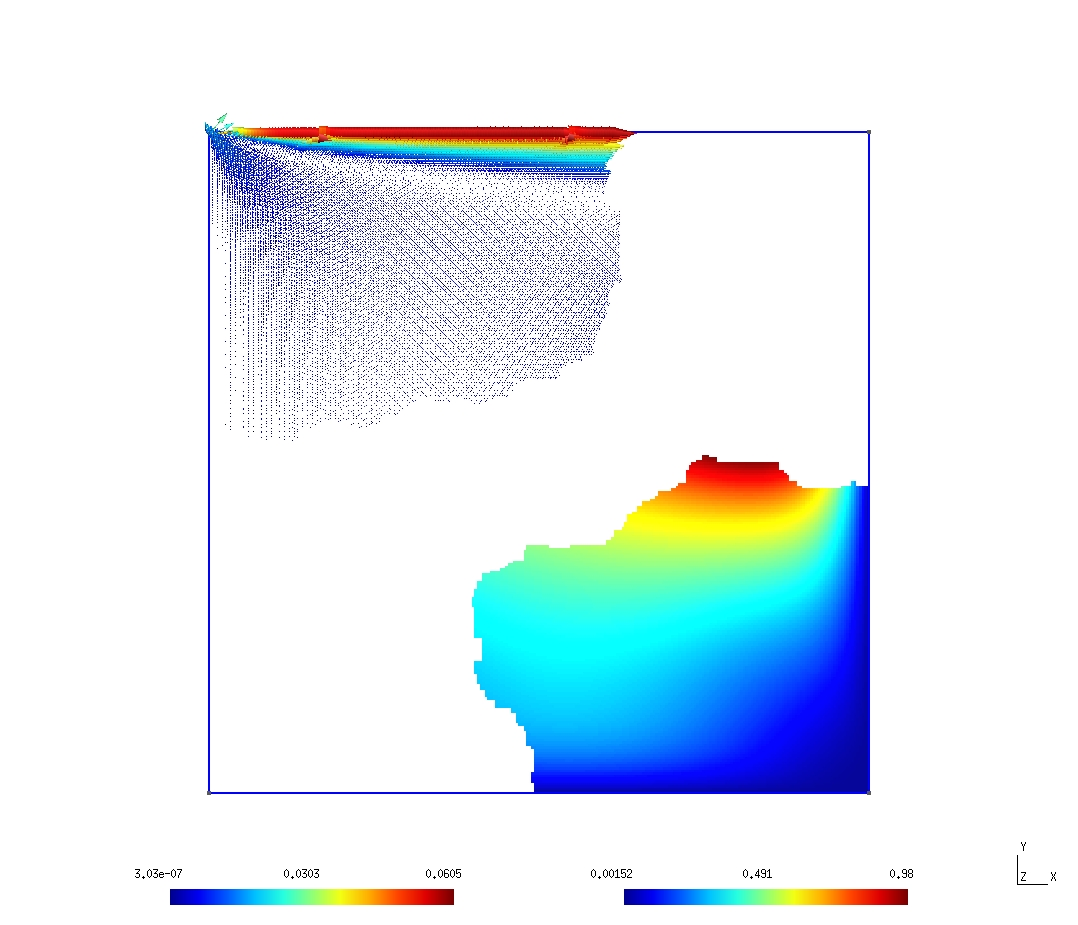
\includegraphics[width=0.99\textwidth]{cavity_2dp_tet_fine}
    \column{0.5\textwidth}
    \centering
    %% \caption {Duct flow}
    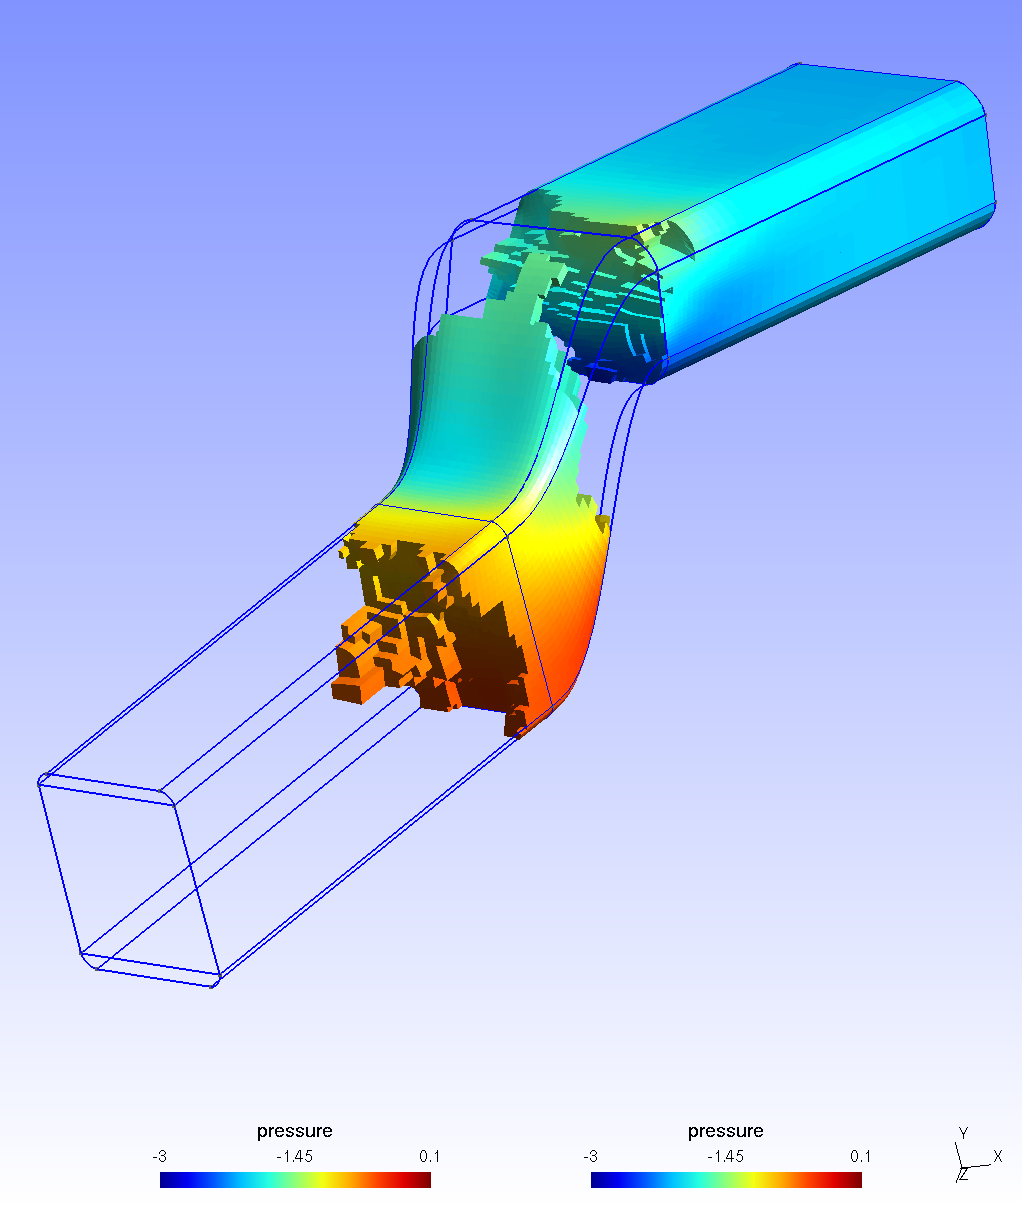
\includegraphics[width=0.85\textwidth]{duct_3d_4p}
  \end{columns}
\end{figure}
\end{frame}


\section{Fundamental Tensions (by analogy)}


\begin{frame}{Complexity - Proliferation}
\begin{figure}
  \centering
  \begin{columns}
    \column{0.5\textwidth}
    \centering
    \caption {[1977] 601 parts, 99 part types}
    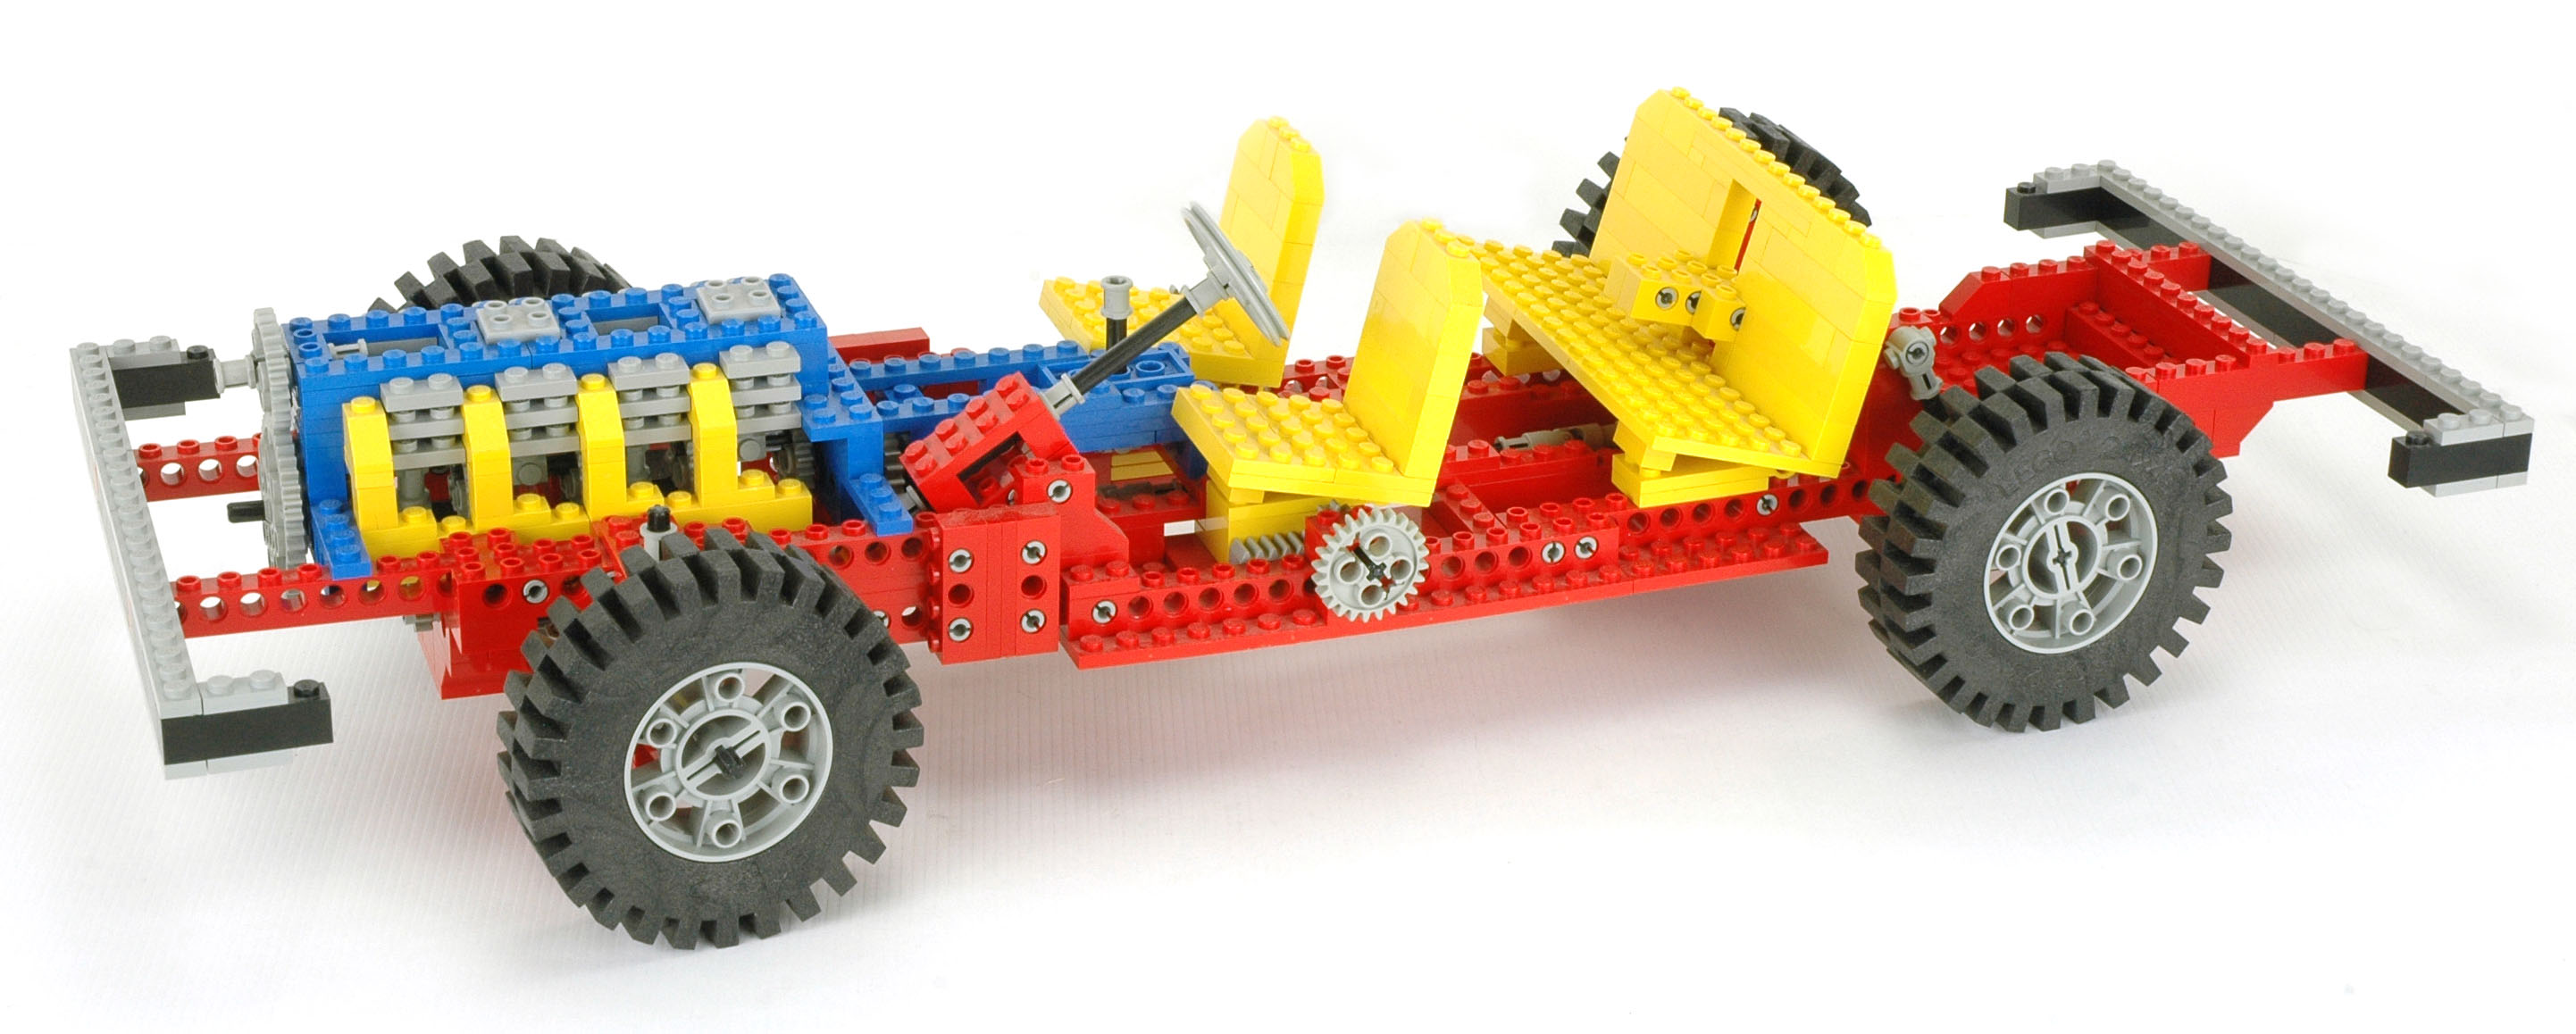
\includegraphics[width=0.9\textwidth]{1977_853_car}
    \column{0.5\textwidth}
    \centering
    \caption {[2016] 3929 parts, 3147 part types}
    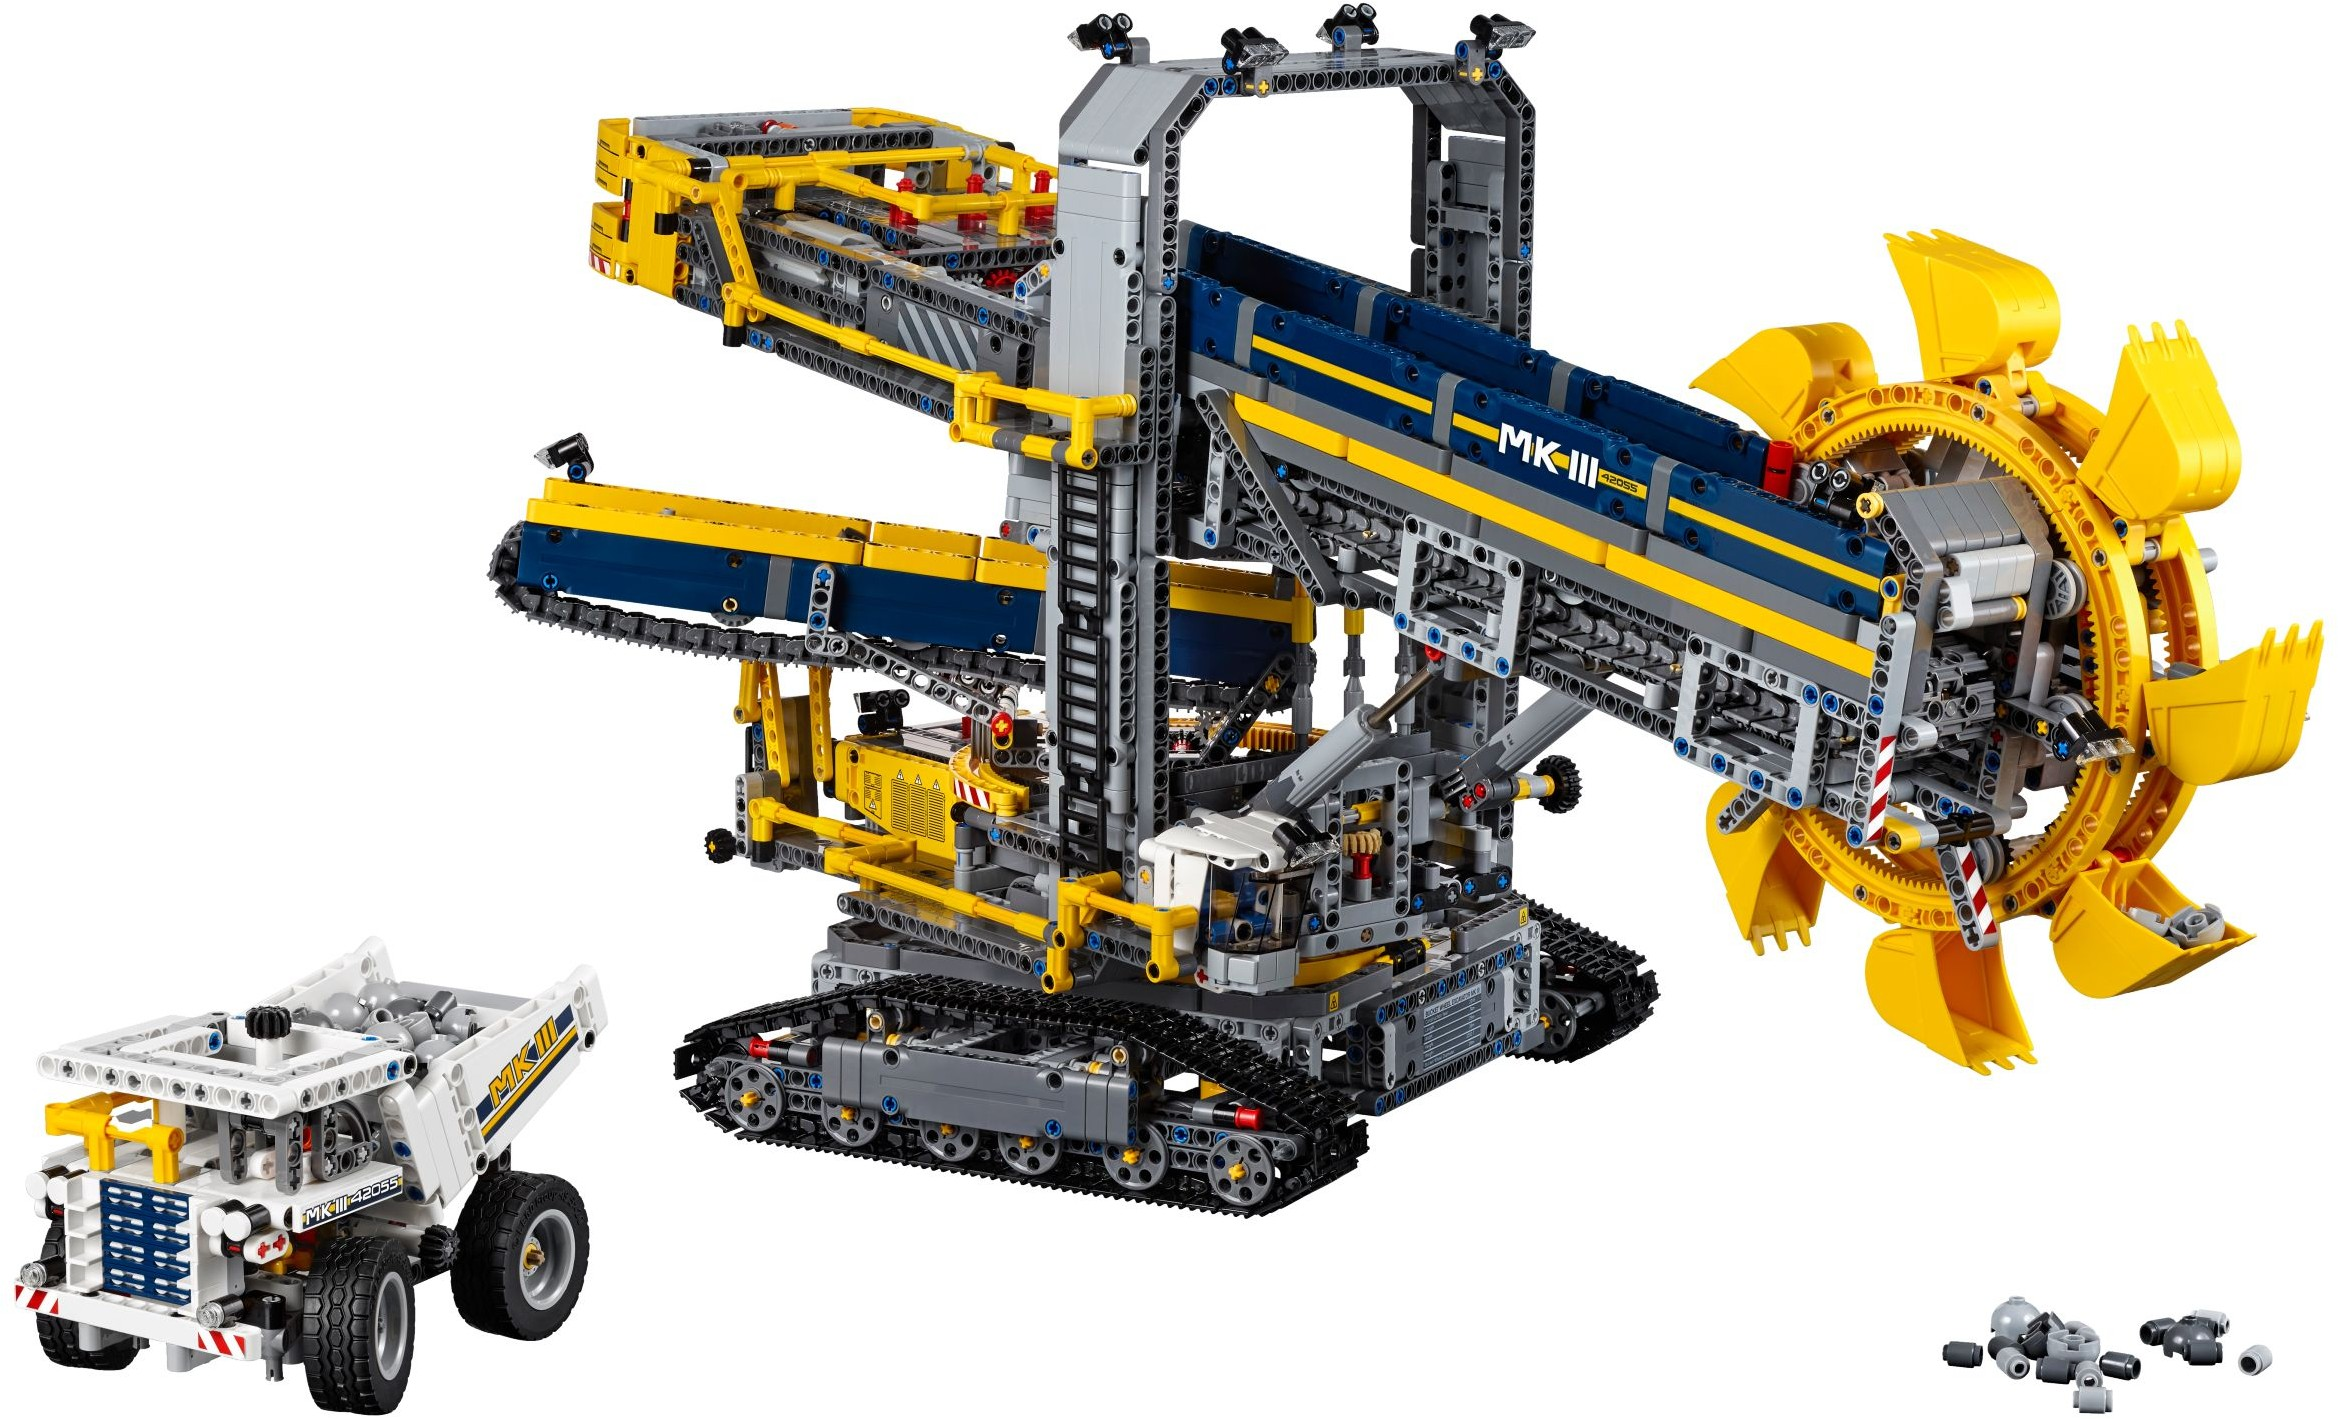
\includegraphics[width=0.9\textwidth]{2016_42055_excavator}
  \end{columns}
\end{figure}
\end{frame}


\begin{frame}{Indirection - Efficiency}
\begin{figure}
  \centering
  \begin{columns}
    \column{0.5\textwidth}
    \centering
    \caption {[1989] Pneumatics\newline flexible, weak}
    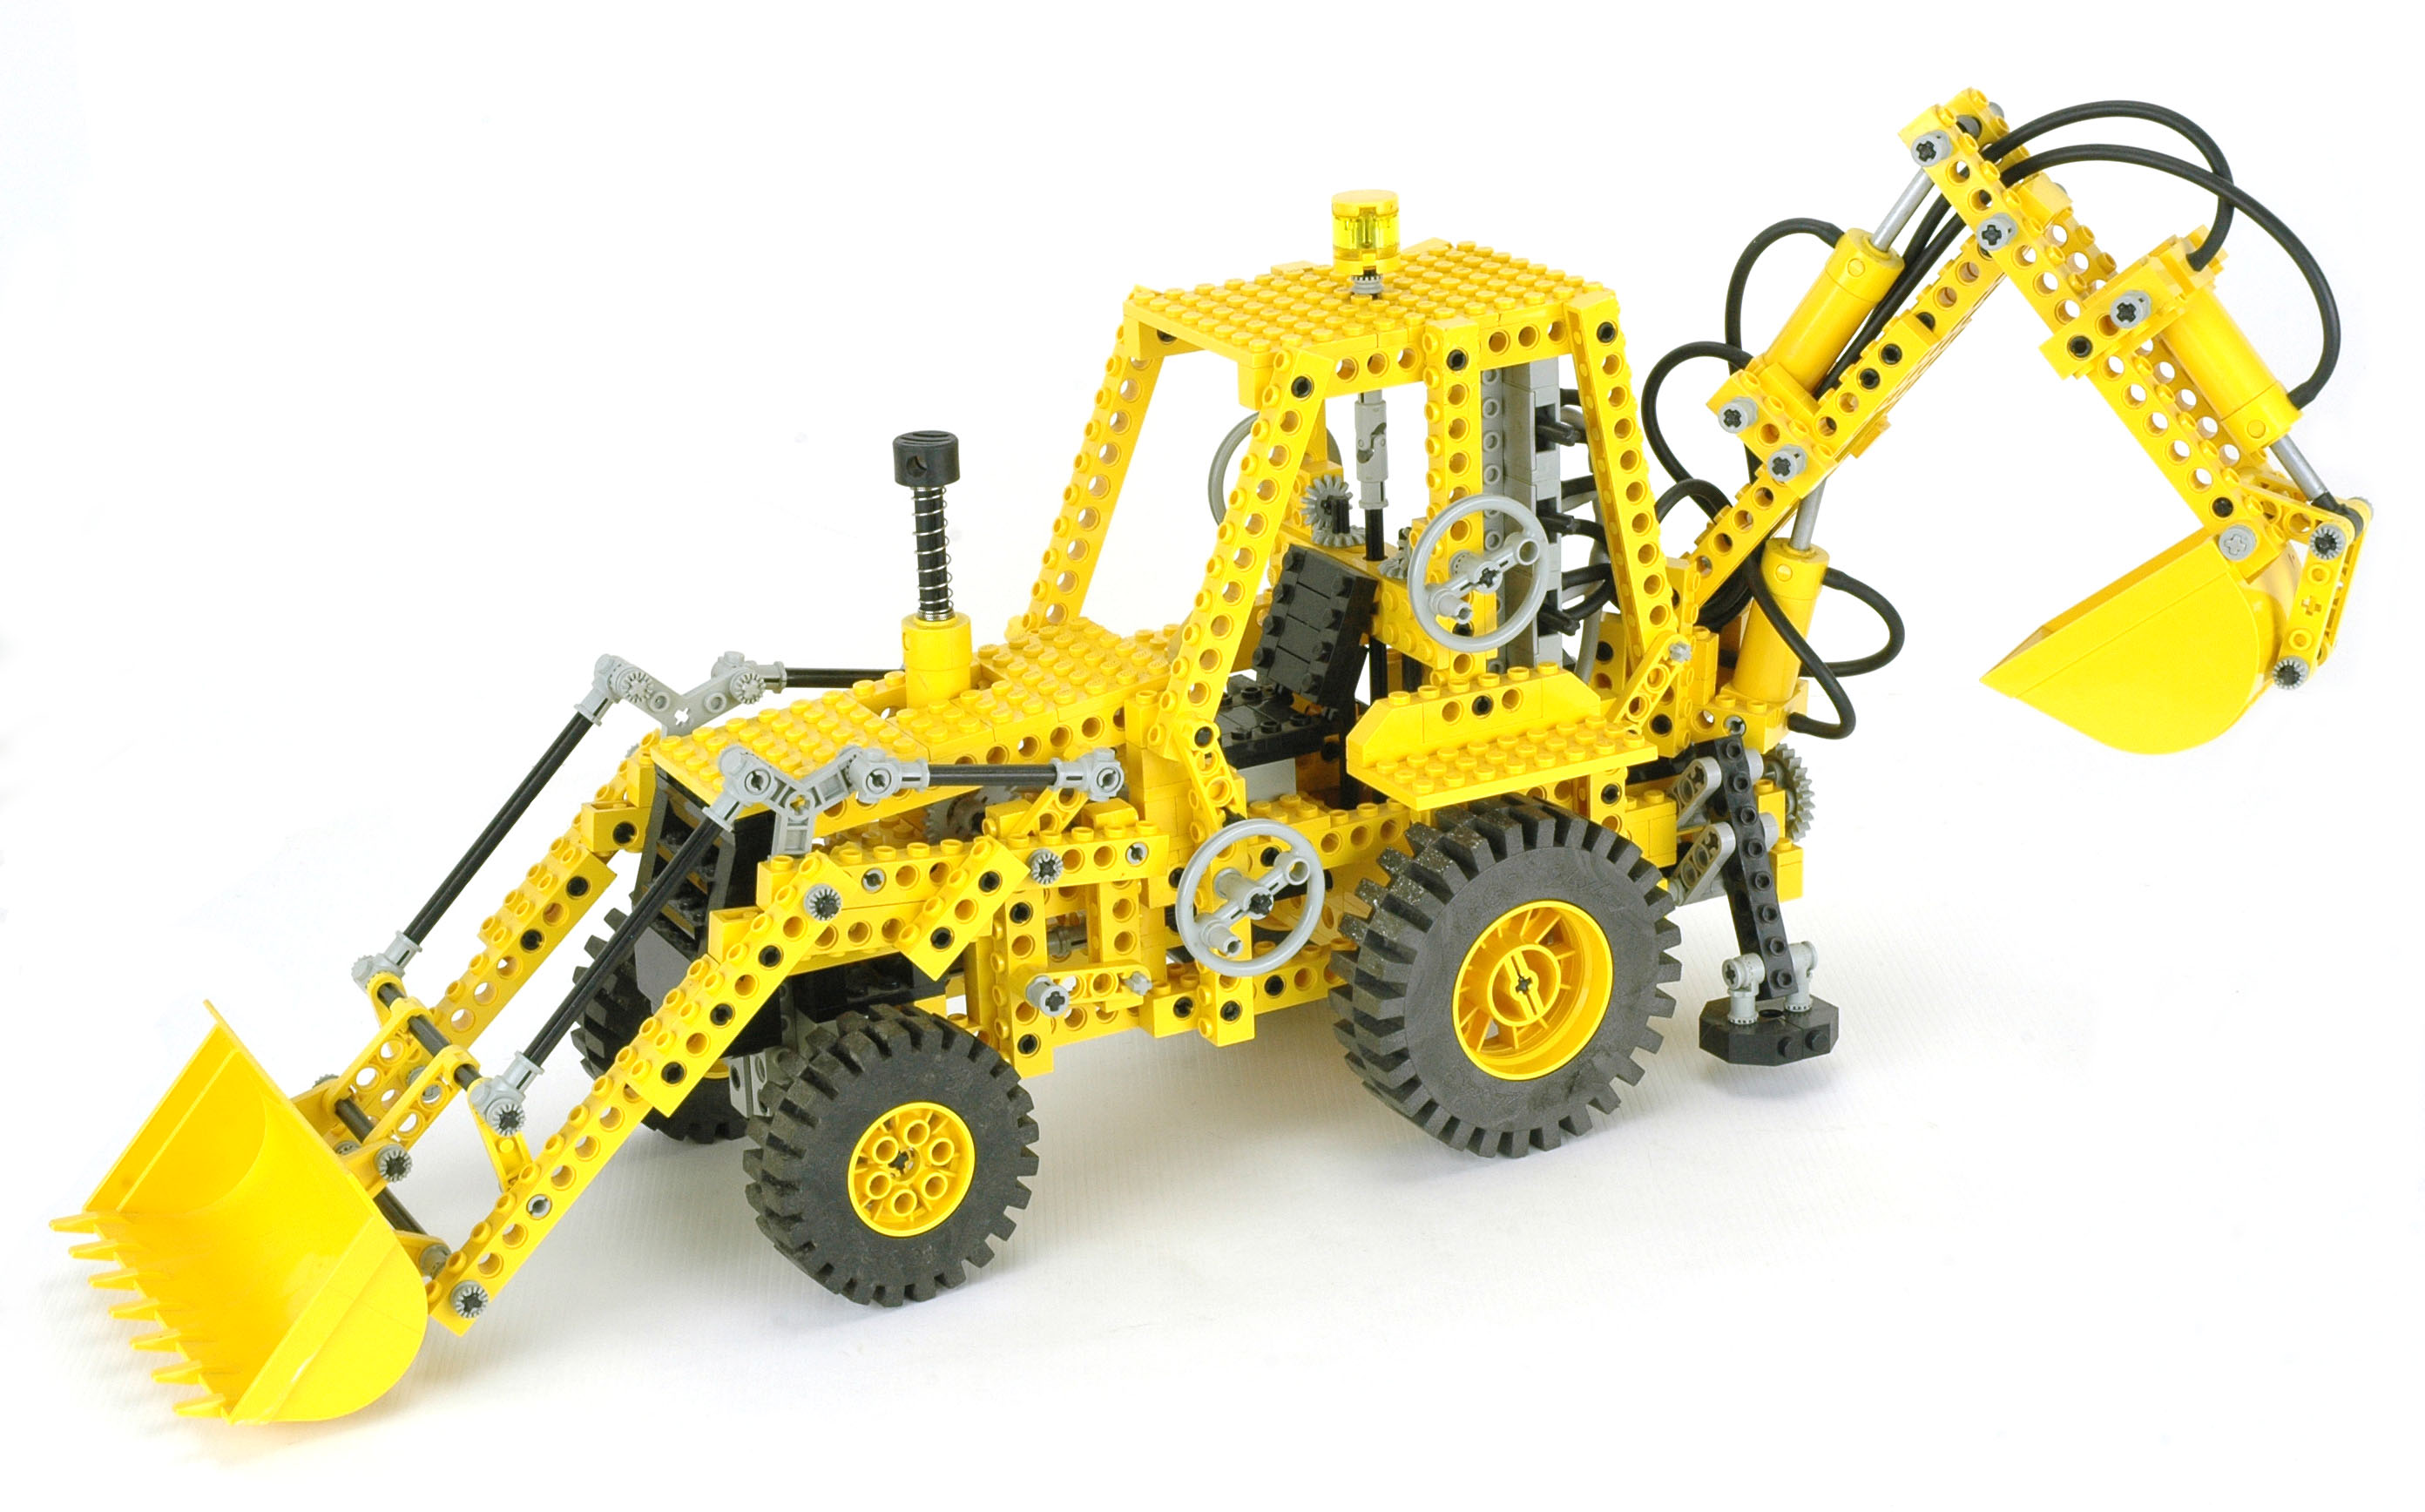
\includegraphics[width=0.9\textwidth]{1989_8862_digger}
    \column{0.5\textwidth}
    \centering
    \caption {[2007] Linear actuators\newline powerful, bulky}
    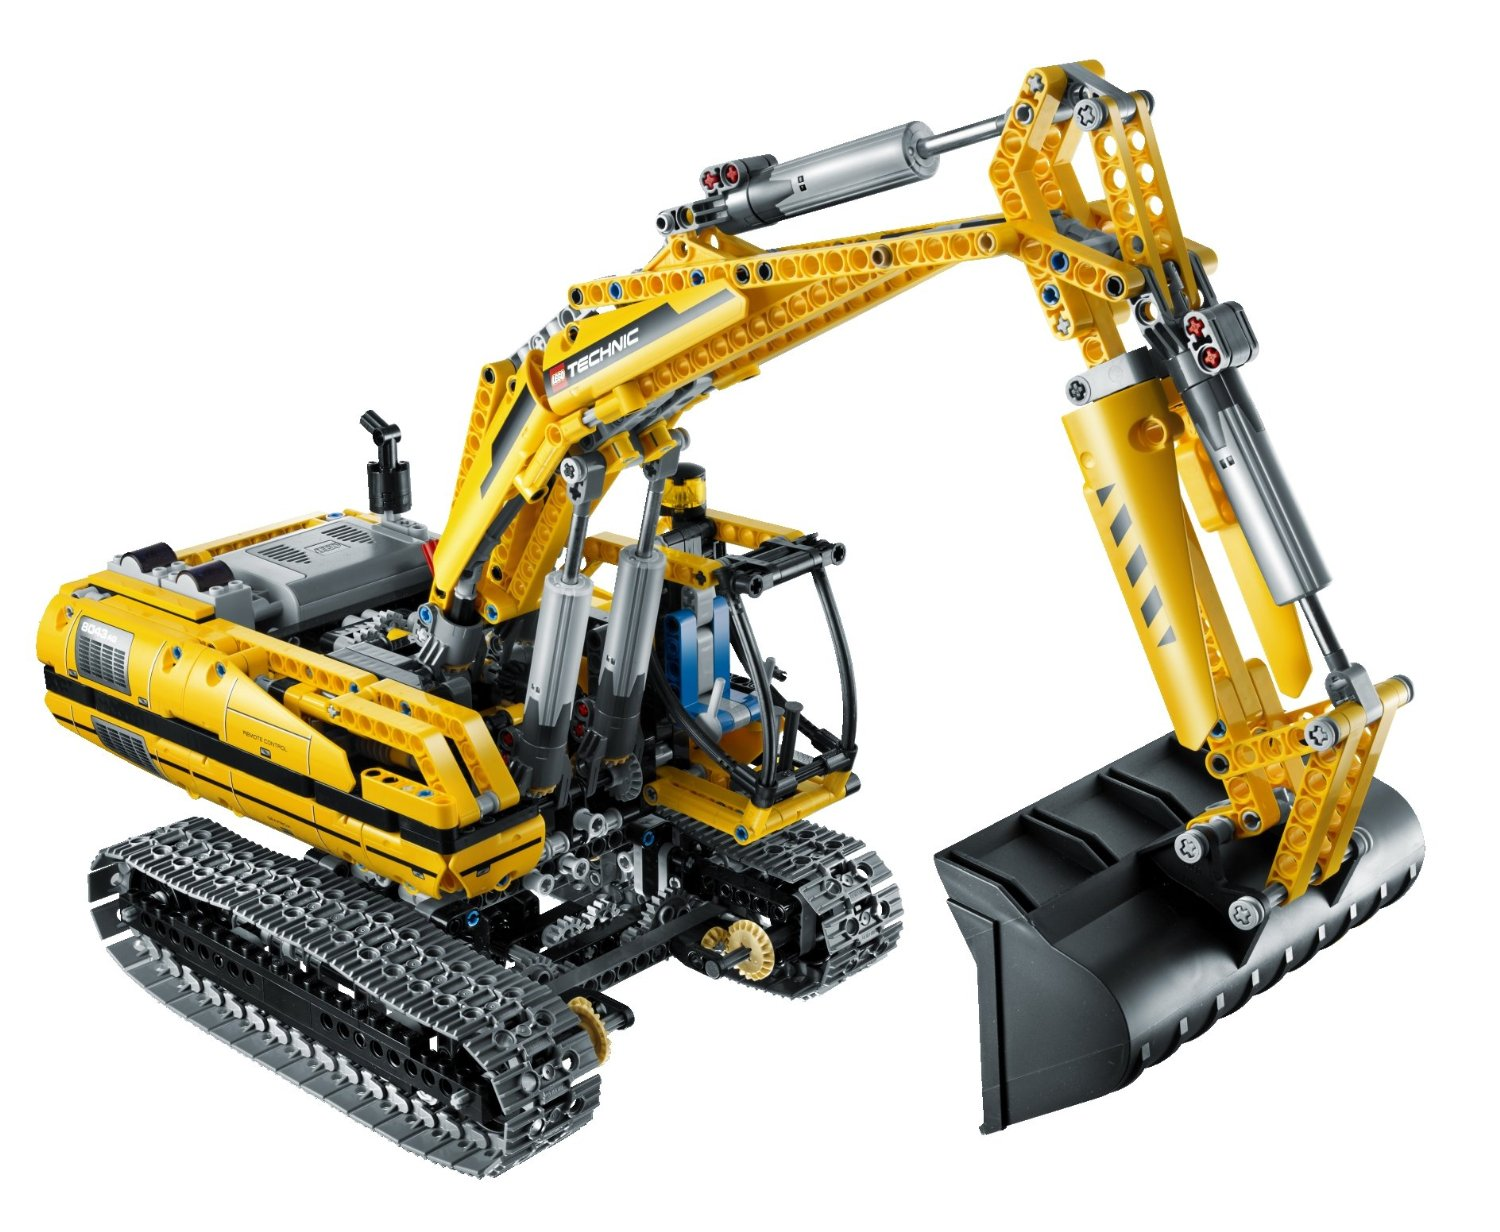
\includegraphics[width=0.9\textwidth]{2010_8043_excavator}
  \end{columns}
\end{figure}
\end{frame}


\section{Artificial Neural Networks - Machine Learning}


\begin{frame}{}
\begin{figure}
  \centering
  \caption {TensorFlow demo}
  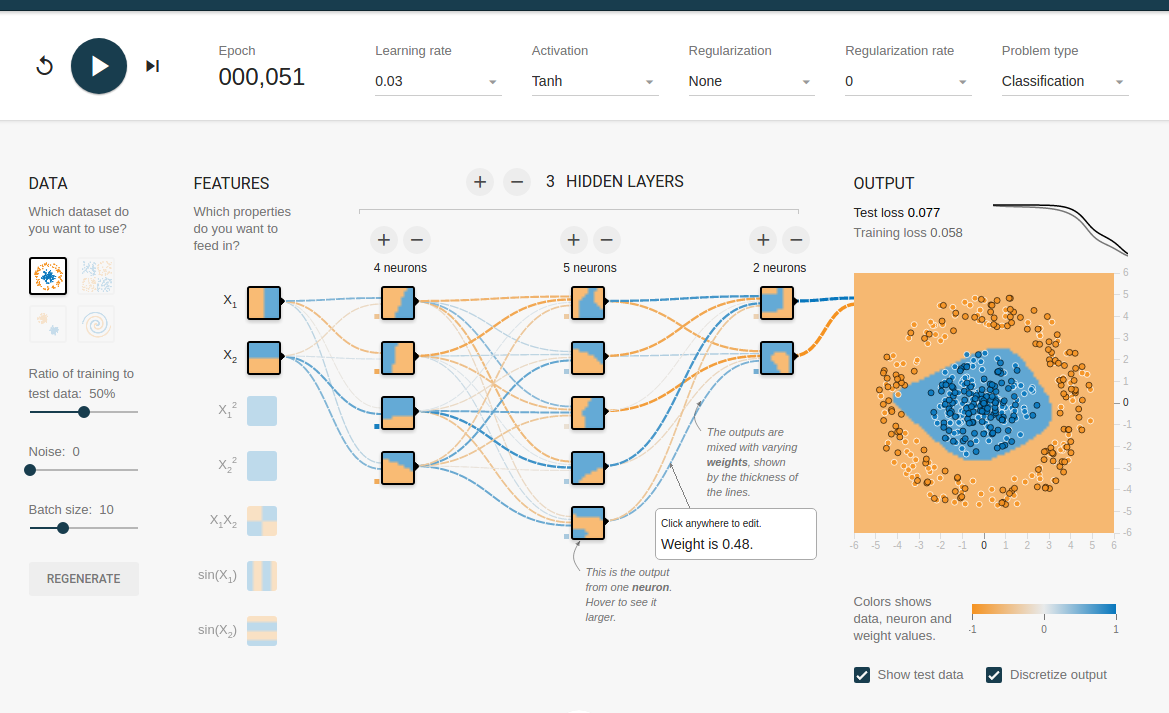
\includegraphics[width=0.9\textwidth]{tensorflow_demo}
\end{figure}
\end{frame}


\begin{frame}
  \frametitle{From the web}
  \begin{enumerate}
  \item Intel 4004 Python emulator
  \item Logisim circuit simulation
  \item Bluebit matrix calculator
  \item Gmsh meshing and post-processing
  \item Flowlab simulation code
  \item TensorFlow demo
\end{enumerate}
\end{frame}

\end{document}
